In, $\triangle{ABC}$ and $\triangle{ADE}$
\begin{align} 
\angle BAD &= \angle EAC \quad (given) \label{eq:solutions/1/26/eq1}
\end{align}
Adding $\angle DAC$ on both side, We get:
\begin{align}
 \angle BAD + \angle DAC &= \angle EAC + \angle DAC \label{eq:solutions/1/26/eqn_2} 
\end{align}

\begin{figure}[!htb]
	\centering
    \centering
\resizebox{\columnwidth}{!}{%\documentclass{article}
%\usepackage[utf8]{inputenc}
%\usepackage{tikz}
%\usetikzlibrary{positioning}
%\begin{document}
	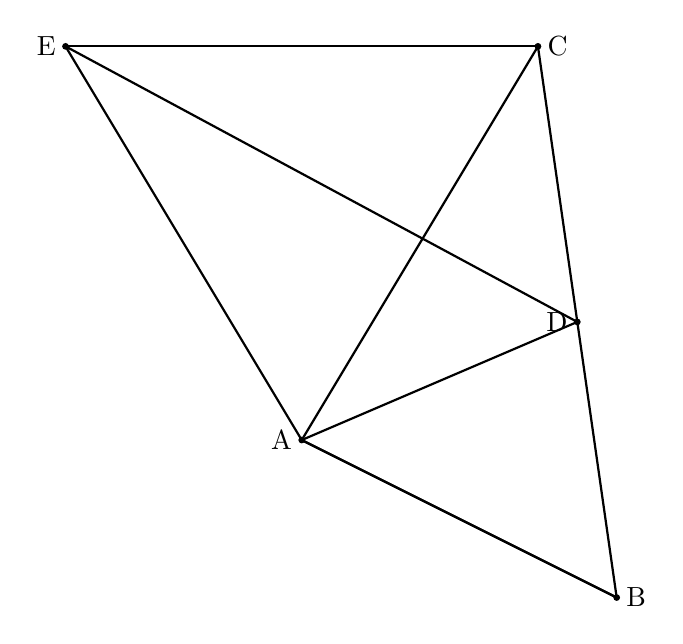
\begin{tikzpicture}
		\draw[black, thick] (0,0) --(4,-2); 
		\draw[black, thick] (4,-2)--(3,5);
		\draw[black, thick] (3,5)--(-3,5);
		\draw[black, thick] (-3,5)--(0,0);
		\draw[black, thick] (0,0)--(3.5,1.5);
		\draw[black, thick] (0,0)--(4,-2);
		\draw[black, thick] (0,0)--(3,5);
		\draw[black, thick] (3.5,1.5)--(-3,5);
		
		\filldraw[black] (0,0) circle (1pt) node[anchor=east] {A};
		\filldraw[black] (4,-2) circle (1pt) 
node[anchor=west] {B};
		\filldraw[black] (3,5) circle (1pt) node[anchor=west] {C};
		\filldraw[black] (-3,5) circle (1pt) node[anchor=east] {E};
		\filldraw[black] (3.5,1.5) circle (1pt)
node[anchor=east] {D};
	\end{tikzpicture}
%\end{document}}
	\caption{Quadrilateral ABCE}
\end{figure}
We have,
\begin{align}
 \angle BAC &= \angle DAE \label{eq:solutions/1/26/eq3}\\
 \implies \cos\angle DAE  &=  \cos\angle BAC \label{eq:solutions/1/26/eq4}
\end{align}
%\begin{align}
%a^2 &= b^2 + c^2-2bc \cos\angle BCA \label{eq:solutions/1/26/eq5}\\
%(\vec B -\vec A)^T(\vec{B}-\vec{C})&=
%\norm{\vec{A}-\vec{B}}^2 - (\vec A -\vec C)^T(\vec{A}-\vec{B})  \label{eq:solutions/1/26/eq6}
%\end{align}
\begin{align}
 \frac{(\vec A -\vec D)^T(\vec{A}-\vec{E})} {\norm{\vec{A}-\vec{D}} \norm{\vec{A}-\vec{E}} } 
 &= \frac{(\vec A -\vec B)^T(\vec{A}-\vec{C})} {\norm{\vec{A}-\vec{B}} \norm{\vec{A}-\vec{C}}}\label{eq:solutions/1/26/eq7}
 \end{align}

We are given AE=AC and we know AD=AB always. Thus, 
\begin{align}
    \norm{\vec{A}-\vec{E}}  &=  \norm{\vec{A}-\vec{C}}\label{eq:solutions/1/26/eq8}\\
    \norm{\vec{A}-\vec{D}}  &=  \norm{\vec{A}-\vec{B}}\label{eq:solutions/1/26/eq9}
\end{align}
Then, from (\ref{eq:solutions/1/26/eq7}), we have,
\begin{align}
(\vec A -\vec D)^T(\vec{A}-\vec{E}) =  (\vec A -\vec B)^T(\vec{A}-\vec{C})\label{eq:solutions/1/26/eq10}
\end{align}
Taking Transpose on both the side:
\begin{align}
((\vec A -\vec D)^T(\vec{A}-\vec{E}))^T =  ((\vec A -\vec B)^T(\vec{A}-\vec{C}))^T\label{eq:solutions/1/26/eq11}\\
(\vec A -\vec E)^T(\vec{A}-\vec{D}) =  (\vec A -\vec C)^T(\vec{A}-\vec{B})\label{eq:solutions/1/26/eq12}
\end{align}
%Using law of cosine (\ref{eq:solutions/1/26/eq6})
%\begin{align}
%\implies \norm{\vec{A}-\vec{D}}^2 - (\vec D -\vec %A)^T(\vec{D}-\vec{E})  \nonumber\\
%\quad \quad =\norm{\vec{A}-\vec{D}}^2 - (\vec B -\vec A)^T(\vec{B}-\vec{C}) \label{eq:solutions/1/26/eq15}\\
% \implies (\vec D -\vec A)^T(\vec{D}-\vec{E}) = (\vec B -\vec A)^T(\vec{B}-\vec{C})\label{eq:solutions/1/26/eq16}\\ 
% \implies \norm{\vec{D} - \vec{A}}\norm{\vec{D} - \vec{E}}\cos\angle ADE \nonumber\\
%\quad \quad= \norm{\vec{B} - \vec{A}}\norm{\vec{D} - \vec{E}}\cos\angle ABC \label{eq:solutions/1/26/eq17}\\
%\implies \norm{\vec{D} - \vec{E}}\cos\angle ADE  = \norm{\vec{B} - \vec{C}}\cos\angle ABC \label{eq:solutions/1/26/eq18}
%\end{align}
We need to prove: $\norm{\vec{B} - \vec{C}} = \norm{\vec{D} - \vec{E}}$ 
%\begin{align}
%& (\vec{D} -\vec{A})^T(\vec{D}-\vec{E}) = (\vec B -\vec A)^T(\vec{B}-\vec{C})\label{eq:solutions/1/26/eq19}
%\end{align}
%Again, By using law of cosine (\ref{eq:solutions/1/26/eq6})
%\begin{multline}
%\implies \norm{\vec{D}-\vec{E}}^2 - (\vec E -\vec D)^T(\vec{E}-\vec{A}) \\
%= \norm{\vec{B}-\vec{C}}^2 - (\vec C -\vec B)^T(\vec{C}-\vec{A})\label{eq:solutions/1/26/eq20}	
%\end{multline}
%\begin{multline}
%\implies \norm{\vec{D}-\vec{E}}^2 - (\norm{\vec{A}-\vec{E}}^2 - (\vec A -\vec D)^T(\vec A -\vec E)) \\
% =\norm{\vec{B}-\vec{C}}^2 - (\norm{\vec{A}-\vec{C}}^2 - (\vec A -\vec B)^T(\vec A -\vec C))	\label{eq:solutions/1/26/eq21}
%\end{multline}
%We are given that AE=AC, AD=AB. Using, (\ref{eq:solutions/1/26/eq12}),(\ref{eq:solutions/1/26/eq13})
%\begin{multline}
%\therefore \norm{\vec{D}-\vec{E}}^2 + (\vec A -\vec D)^T(\vec{A}-\vec{E}) = \\ \norm{\vec{B}-\vec{C}}^2 + (\vec A -\vec B)^T(\vec{A}-\vec{C}) \label{eq:solutions/1/26/eq22}	
%\end{multline}
%\begin{multline}
%\implies \norm{\vec{D}-\vec{E}}^2+ \norm{\vec{A}-\vec{D}}\norm{\vec{A}-\vec{E}}\cos \angle DAE = \\
% \norm{\vec{B}-\vec{C}}^2+\norm{\vec{A}-\vec{B}} \norm{\vec{A}-\vec{C}}\cos \angle BAC \label{eq:solutions/1/26/eq23}	
%\end{multline}
%From the question, $\angle DAE = \angle BAC$ and $\norm{\vec{A}-\vec{E}} = \norm{\vec{A}-\vec{C}}$. We also know $\norm{\vec A -\vec D}= \norm{ \vec A- \vec B}$. 
%Thus, from (\ref{eq:solutions/1/26/eq23}), we get,
\begin{multline}
\implies \norm{\vec{B}-\vec{C}}^2 - \norm{\vec{D}-\vec{E}}^2=\\
(\vec B -\vec C)^T(\vec{B}-\vec{C})-(\vec D -\vec E)^T(\vec{D}-\vec{E})\label{eq:solutions/1/26/eq13}
\end{multline}
\begin{multline}
=((\vec A -\vec C)-(\vec A -\vec B))^T((\vec A -\vec C)-(\vec A -\vec B))\\-((\vec A -\vec E)-(\vec A -\vec D))^T((\vec A -\vec E)-(\vec A -\vec D))\label{eq:solutions/1/26/eq14}
\end{multline}
\begin{multline}
=\norm{\vec{A}-\vec{C}}^2 + \norm{\vec{A}-\vec{B}}^2- (\vec A -\vec B)^T(\vec{A}-\vec{C})-(\vec{A}-\vec{C})^T(\vec{A}-\vec{B})\\
-\norm{\vec{A}-\vec{E}}^2 - \norm{\vec{A}-\vec{D}}^2+ (\vec A -\vec D)^T(\vec{A}+\vec{E})+(\vec{A}-\vec{E})^T(\vec{A}-\vec{D})\label{eq:solutions/1/26/eq15}
\end{multline}
Thus, from (\ref{eq:solutions/1/26/eq8}), (\ref{eq:solutions/1/26/eq9}), (\ref{eq:solutions/1/26/eq10}) and (\ref{eq:solutions/1/26/eq12})
\begin{align}
& \norm{\vec{B}-\vec{C}}^2 - \norm{\vec{D}-\vec{E}}^2=0\label{eq:solutions/1/26/eq16}\\ 
& \implies \norm{\vec{B}-\vec{C}}^2 = \norm{\vec{D}-\vec{E}}^2 \label{eq:solutions/1/26/eq17}\\
	& \therefore\norm{\vec{B}-\vec{C}} = \norm{\vec{D}-\vec{E}}\label{eq:solutions/1/26/eq18}
\end{align}
Hence, BC=DE

